\begin{frame}
	\frametitle{$\DPLL$-алгоритмы}

   	\onslide<1->{
   	\tikzstyle{vertex2} = [opacity = 0]
   	\tikzstyle{vertex3} = [opacity = 0]
    \tikzstyle{vertex4} = [opacity = 0]
   	\tikzstyle{vertex5} = [opacity = 0]
    \tikzstyle{vertex9} = [opacity = 0]
    \tikzstyle{vertex11} = [opacity = 0]
}
\only<2->{\tikzstyle{vertex2} = [opacity = 1]}
\only<3->{\tikzstyle{vertex3} = [opacity = 1]}
\only<4->{\tikzstyle{vertex4} = [opacity = 1]}
\only<5->{
  	\tikzstyle{vertex5} = [opacity = 1]
    \tikzstyle{vertex9} = [opacity = 1]
}

\tikzstyle{end} = [circle, minimum size = 0.6cm, draw, inner sep = 0.1pt]
            
\tikzstyle{level 1} = [level distance = 1.5cm, sibling distance = 5cm]
\tikzstyle{level 2} = [sibling distance = 2cm]
    
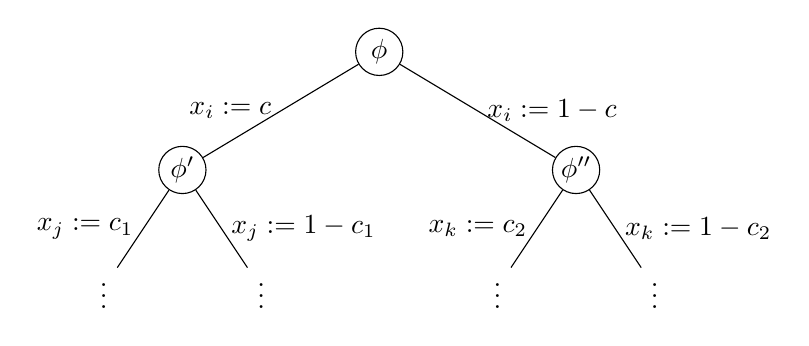
\begin{tikzpicture}[label distance = 8mm]
	\node [end] (z){$\phi$}
       	child [vertex2] {node [end] (b) {$\phi'$}
			child [vertex3]{
	           	node {$\vdots$}
                edge from parent
	  	        node[left] {$x_{j} := c_1$}
            }
		    child [vertex4]{
               	node {$\vdots$}
                edge from parent
	   	        node[right] {$x_{j} := 1 - c_1$}
            }
           	edge from parent
            node[left] {$x_{i} := c$}
        }
        child [vertex5] {node [end] (c) {$\phi''$}
           	child [vertex9]{
               	node {$\vdots$}
                edge from parent
	            node[left] {$x_{k} := c_2$}
            }
		    child [vertex9]{
               	node {$\vdots$}
                edge from parent
	            node[right] {$x_{k} := 1 - c_2$}
            }
            edge from parent
	   	    node[right] {$x_{i} := 1 - c$}
        };
\end{tikzpicture}

    
	\pause
    \pause
    \pause
    \pause
    \pause
    \begin{itemize}
        \item Процедура $\mathbf{A}$ выбирает переменную для расщепления.
    	\pause
	    \item Процедура $\mathbf{B}$ выбирает первое значение.
    	\pause
    	\item Правила упрощения:
	    \begin{itemize}
            \item удаление единичного дизъюнкта;
        	\item чистые литералы.
    	\end{itemize}
    \end{itemize}

\end{frame}


\begin{frame}
    \frametitle{$\DPLL$-алгоритмы}

    \begin{itemize}
        \item $\SAT$-солверы основаны на алгоритмах расщепления ($CDCL$ не укладываются в данную модель).
        \item Оптимальность на выполнимых формулах.
	\end{itemize}

    \pause
    \begin{block}{Утверждение}
   		Если $\P = \NP$, то существует верхняя полиномиальная оценка на время работы $\DPLL$-алгоритма на \alert{выполнимых формулах}.        
    \end{block}

\end{frame}

\begin{frame}
    \frametitle{Нижние оценки}

    \pause
	\begin{itemize}
		\item Невыполнимые формулы
		\begin{itemize}
            \item{} Экспоненциальный нижние из оценки следуют из нижних оценок для резолюции.
			\item{} [Tseitin, 1968] ... [Pudlak, Implagliazzo, 2000].
		\end{itemize}
        \pause
		\item Выполнимые формулы
		\begin{itemize}
			\item Обращение функции соответствует выполнимой формуле..
            \pause
            \item{} [Nikolenko~2002], [Achilioptas, Beame, Molloy~2003-2004] экспоненциальные нижние оценки на специфические алгоритмы.
            \item{} [Alekhnovich, Hirsch, Itsykson~2005] экспоненциальные нижние оценки на ``близорукие'' и ``пьяные'' алгоритмы.
            \pause
            \item{}  Экспоненциальные нижние оценки на время обращения функции Голдрейха для близоруких [J. Cook et al.~2009,
				2014] и пьяных [Itsykson~2010] алгоритмов.
		\end{itemize}
	\end{itemize}
\end{frame}

\begin{frame}
	\frametitle{Пьяные и близорукие алгоритмы}
    \pause

    \begin{definition}
        Пьяный алгоритм:
        \begin{itemize}
	        \item $\mathbf{A}$~--- произвольная;
	        \item $\mathbf{B}$~--- случайный бит.
        \end{itemize}
    \end{definition}

    \pause
    \begin{definition}
        Близорукая процедура:
        \pause
        \begin{itemize}
	        \item видит структуру формулы;
        	\pause
        	\item не видит отрицаний;
        	\item<6-> запрашивает отрицания в $K = n^{1 - \epsilon}$ клозах.
        \end{itemize}
    \end{definition}

    \pause
    $\begin{array}{l}
        (x_1 \vee x_3 \vee x_5) \\
        \alert<7->{(x_2 \vee x_3)} \\
        (x_2 \vee x_4 \vee x_5) \\
        \alert<7->{(x_1 \vee x_4 \vee x_6)} \\
    \end{array}
    \pause
    \pause
    \pause
    \Rightarrow
    \begin{array}{l}
        (x_1 \vee x_3 \vee x_5) \\
        (x_2 \vee \alert{\neg} x_3) \\
        (x_2 \vee x_4 \vee x_5) \\
        (x_1 \vee \alert{\neg} x_4 \vee x_6) \\
    \end{array}$
    
\end{frame}

\begin{frame}
	\frametitle{Функция Голдрейха}
	$f:\{0, 1\}^n \rightarrow \{0, 1\}^n$

    \pause

    \begin{columns}
    	\begin{column}{5.5cm}
            \tikzstyle{end} = [circle, minimum width = 4pt, fill, inner sep = 1pt,
	opacity = 1]
\tikzstyle{start} = [circle, inner sep = 1pt, opacity = 1]
            
\tikzstyle{level 1} = [level distance = 0.1cm, sibling distance = 0.4cm]
\tikzstyle{level 2} = [level distance = 0.45cm]
\tikzstyle{level 3} = [level distance = 1cm]
\tikzstyle{level 4} = [level distance = 0.4cm]

\begin{tikzpicture}[grow = right]
    \node [start]{}
    	child {
        	node [start] (xn) {$x_{n}$}
            	child [end]{
                	node [end] (xvn){}
                    	child [end]{
                        	node [end] (yvn){}
                            	child [start]{
                                	node [start] (yn){}
                                    edge from parent [opacity = 1]
                                }
                            edge from parent [opacity = 0]
                        }
                    edge from parent [opacity = 1]
                }
            edge from parent [opacity = 0]
        }
    	child foreach \i in {3, 2, 1}{
	    	node [start] {}
            	child [start]{
                	node [start] {.}
                    	child [start]{
                        	node [start] {.}
                            edge from parent [opacity = 0]
                        }
                    edge from parent [opacity = 0]
                }
            edge from parent [opacity = 0]
        }
    	child foreach \i in {3, 2, 1}{
	    	node [start] (x\i) {$x_{\i}$}
            	child [end]{
                	node [end] (xv\i){}
                    	child [end]{
                        	node [end] (yv\i){}
                            	child [start]{
                                	node [start] (y\i){}
                                    edge from parent [opacity = 1]
                                }
                            edge from parent [opacity = 0]
                        }
                    edge from parent [opacity = 1]
                }
            edge from parent [opacity = 0]
        };

    \path [draw = red, opacity = 1](xv2) -- (yv2);
    \path [draw = red, opacity = 1](xv3) -- (yv2);
    \path [draw = red, opacity = 1](xvn) -- (yv2);
    \node at (xvn.south) [below = 0.05cm] {$X$};
    \node at (yvn.south) [below = 0.05cm] {$Y$};
    \node <.(2)-> at (y2.east) [right = 0.1cm] {$x_{2} \oplus x_{3}
	    \oplus \dots \oplus x_{n}$};
\end{tikzpicture}

        \end{column}

        \pause
        \pause
        \begin{column}{5.5cm}
            \begin{itemize}
	            \item $G(X, Y, E)$~--- двудольный граф;
            	\pause
                \item $\forall y \in Y ~~ deg(y) = d$
            	\pause
            	\item $d$~--- константа.
            \end{itemize}
        \end{column}
	\end{columns}
    

    \pause
    \begin{theorem}
		Существует такая \alert{явная} конструкция графа $G$ и такой нелинейный предикат $P$, что любой близорукий или пьяный
        $\DPLL$-алгоритм делает $2^{n^{\Omega(1)}}$ шагов на ``$f_{G, P}(x) = f_{G, P}(a)$'' для почти всех $a \in \{0, 1\}^n$.
	\end{theorem}
\end{frame}